\documentclass{cheatsheet}

\doctitle{Chemistry Cheatsheet}
\author{Noa Sendlhofer \& Christian Leser \\ nsendlhofer \& cleser}

\begin{document}
\section{1. Basics} %Noa
	\subsection{1.1 Unit conversions}
	\begin{itemize}
		\itemsep0em
		\raggedright
  		\item \textbf{Energy:} $1eV=1.602\cdot 10^{-19}J$,    $1cal=4.18J$
    	\item \textbf{Pressure:} $P = \frac{F}{A} = \rho \cdot h \cdot g$\\ $1 \textrm{atm} = 760mm \; \textrm{Hg} = 760 \textrm{torr} = 101'325 \textrm{Pa} = 1.01325 \textrm{bar}$\\ Manometer: $P = P_{atm}\pm \rho g h$
    	\item \textbf{Force:} $F = m \cdot g, \; m = \rho \cdot V$
		\item \textbf{Amount of substance:} $1 \textrm{mol} = 6.022\cdot 10^{23} \textrm{(Avogadro)}$
    	\item \textbf{Length:} $1\text{Å}=10^{-10}m$
    	\item \textbf{STP; } $0\tccentigrade = 273.15K, \; 1atm; \; V_m = 22.41L$
	\end{itemize}

\subsection{1.2 General}
    \begin{itemize}
		\itemsep0em
        \item \textbf{Kinetic energy:} $E_{kin} = \frac{1}{2} \cdot m \cdot v^2$
        \item \textbf{Potential energy:} $E_{pot} = m \cdot g \cdot \Delta h$
        \item \textbf{electrostatic:} $E_{el}=\frac{\kappa Q_1Q_2}{d^2}$\quad $\kappa = \frac{1}{4\pi \epsilon_0}$
        \item \textbf{Photon energy: } $E_\gamma = h\cdot f = \frac{h\cdot c}{\lambda}$
        \item \textbf{De Broglie wavelength: } $\lambda = \frac{h}{m\cdot v}$
    \end{itemize}
    	
\subsection{1.3 Trends in the periodic table of elements}
	\begin{itemize}
		\itemsep0em
    	\item \textbf{Ionisation energy: }The ionization energy is the quantity of energy that an isolated, gaseous atom in the ground electronic state must absorb to discharge an electron, resulting in a cation.
    	\item \textbf{Electron affinity: }Electron affinity is defined as the change in energy (in kJ/mole) of a neutral atom (in the gaseous phase) when an electron is added to the atom to form a negative ion.
    	\item \textbf{Electronnegativity:} Electronegativity is a measure of an atom's ability to attract shared electrons to itself.
	\end{itemize}
	\centerline{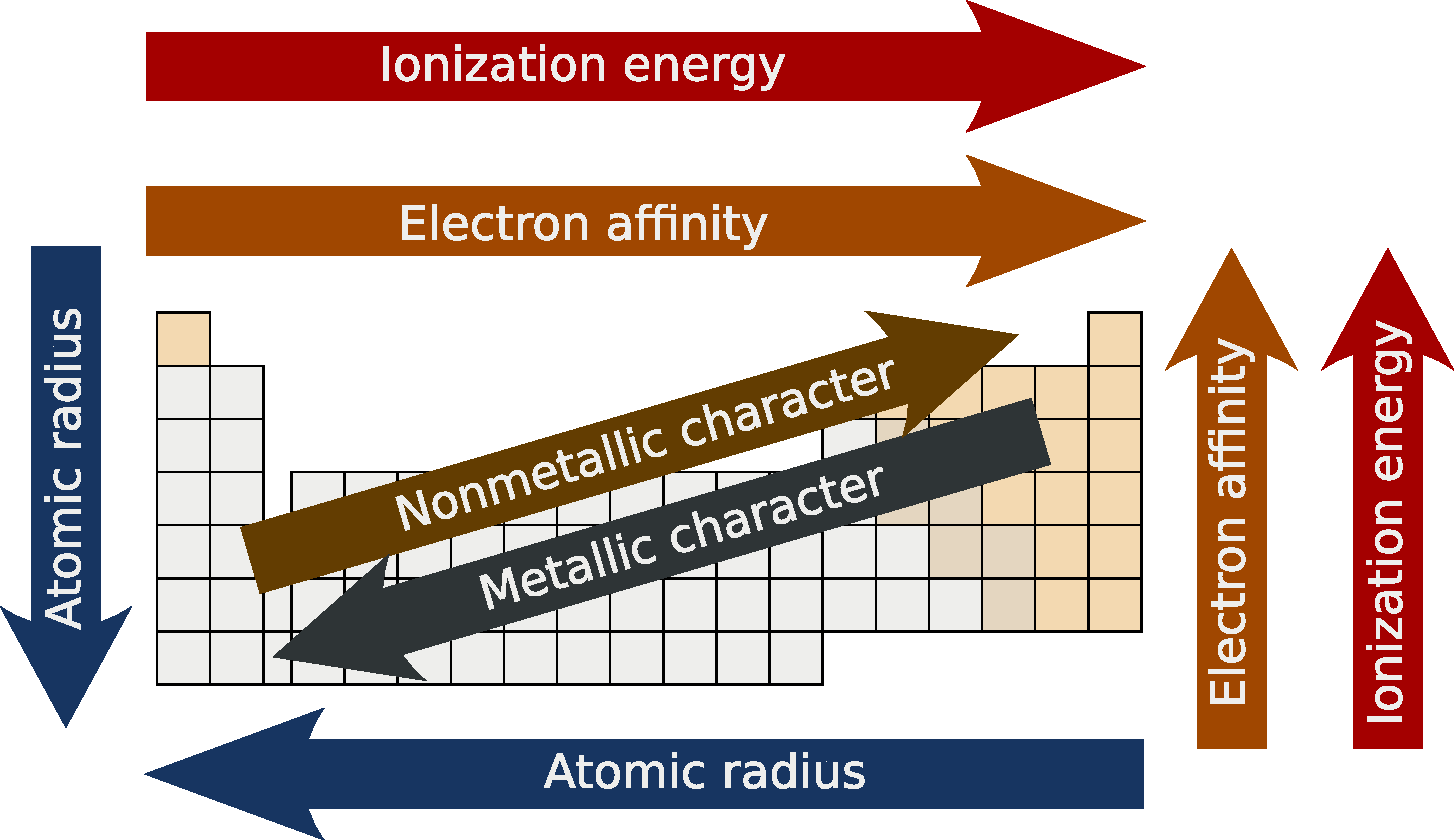
\includegraphics[width=0.65\linewidth]{src/1_Basics/Periodic_trends.pdf}}
	\vspace*{0.5em}

\section{2. Atoms} %Christian
	\subsection{Quantum mechanics}
	\subsection{2.1 Quantum mechanics}
    \begin{scriptsize}
        \begin{tabular}{c c}
            Atomic mass = total mass & Atomic weight = average atomic mass (isotopes)\\
            Atomic number = \#protons & mass number = \#protons + \#neutrons
        \end{tabular}
    \end{scriptsize}
        \vspace*{0.0em}
        
        Heisenbergs uncertainty principle $\Delta x \cdot \Delta p \geq \frac{h}{4 \cdot \pi}$ Due to duality of electrons (acting like waves and elementary entities at the same time), impossible to exactly describe position and momentum simultaneously.\\
        \textbf{Effective nuclear charge (approx.):}   $Z_{eff} = Z-S$\\
        $Z$ = \#protons, $S$ = \#$e^-$ on all full shells
        \vspace{1mm}\\
        In periodic table: $Z_{eff}$ increases from left to right $\rightarrow$ electrons are more attracted and hence atomic radius is smaller, the further right in the periodic table. ($e^-$ repulsion vs. nuclear charge)
        \vspace*{0.0em}
	\subsection{Orbitals}
	\subsection{2.2 Orbitals}
  \begin{minipage}{0.99\linewidth}
    \begin{minipage}{0.33\linewidth}
      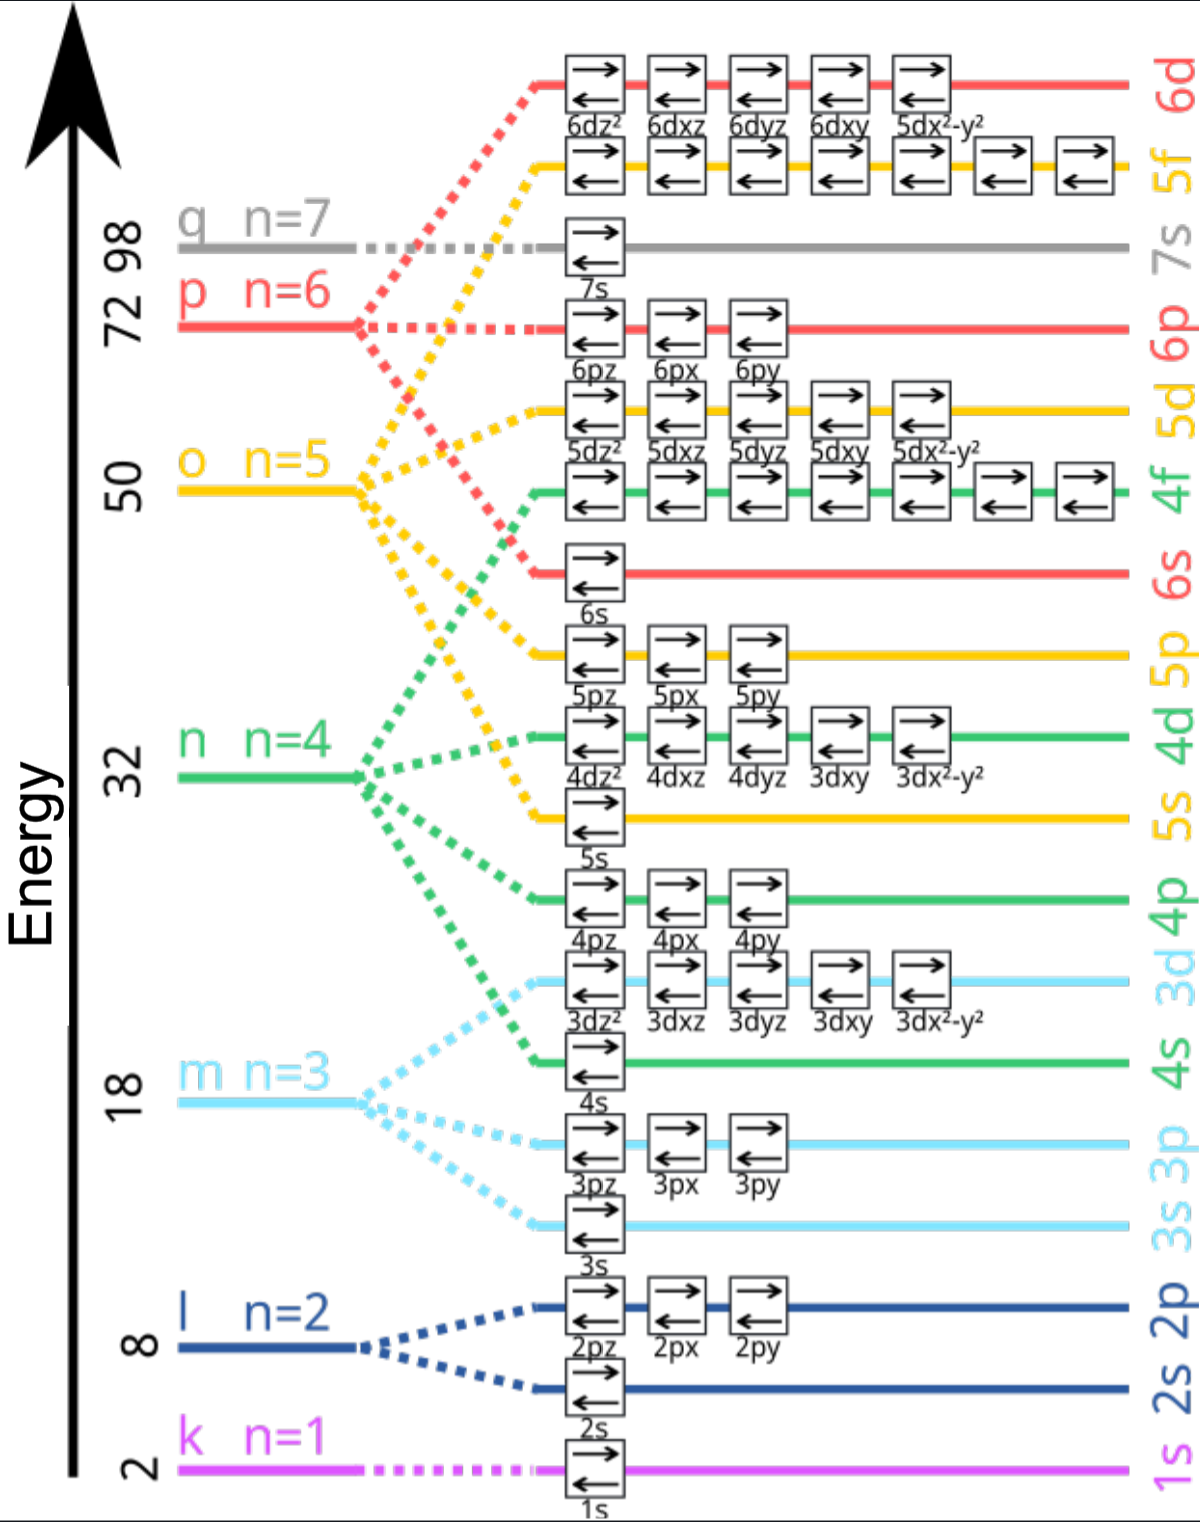
\includegraphics[width = 2.3cm]{src/2_Atoms/images/Energieniveau.png}
    \end{minipage}
    \begin{minipage}{0.52\linewidth}
      \begin{scriptsize}
        \begin{center}
            \begin{tabular}{|p{0.3mm}|c|p{0.07\textwidth}|c|c|}
                \multicolumn{1}{p{0.3mm}}{n} & \multicolumn{1}{c}{l} & \multicolumn{1}{p{0.07\textwidth}}{\rotatebox{90}{\pbox{1.5cm}{subshell\\ designation}}} & \multicolumn{1}{c}{$m_i$} & \multicolumn{1}{c}{$m_s$} \\ [0.5ex]
                \hline
                1 & 0, s & 1s                                  & 0                      & $\pm 1/2$ \\ 
                \hline
                2 & 0, s & 2s                                  & 0                      & $\pm 1/2$ \\
                  & 1, p & 2p                                  & 1, 0, -1               & $\pm 1/2$ \\
                \hline
                3 & 0, s & 3s                                  & 0                      & $\pm 1/2$ \\
                  & 1, p & 3p                                  & 1, 0, -1               & $\pm 1/2$ \\
                  & 2, d & 3d                                  & 2, 1, 0, -1, -2        & $\pm 1/2$ \\
                \hline
                4 & 0, s & 4s                                  & 0                      & $\pm 1/2$ \\
                  & 1, p & 4p                                  & 1, 0, -1               & $\pm 1/2$ \\
                  & 2, d & 4d                                  & 2, 1, 0, -1, -2        & $\pm 1/2$ \\
                  & 3, f & 4f                                  & 3, 2, 1, 0, -1, -2, -3 & $\pm 1/2$ \\
                \hline
            \end{tabular}
        \end{center}
        \end{scriptsize}
    \end{minipage}
  \end{minipage}
        
    \begin{itemize}
        \itemsep0em
        \item \textbf{n}: principal quantum number $\rightarrow$ size of orbital
        \item \textbf{l}: angular quantum number $\rightarrow$ shape of orbital
        \item $\boldsymbol{m_l}$: magnetic quantum number $\rightarrow$ orientation of orbital
        \item $\boldsymbol{m_s}$: spin quantum number
    \end{itemize}
    \vspace*{-0.9em}
    
    \begin{minipage}{0.99\linewidth}
      \begin{minipage}{0.45\linewidth}
        \centerline{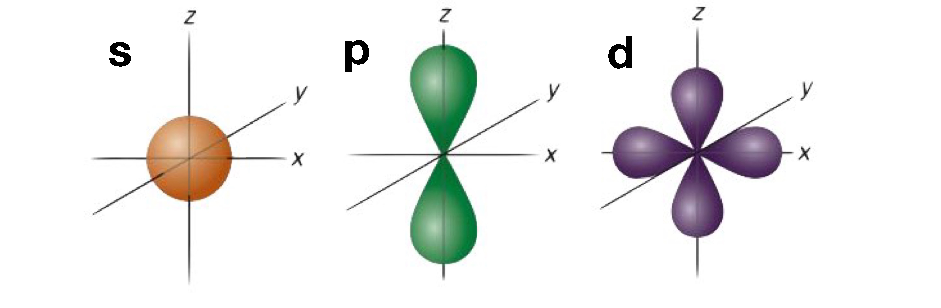
\includegraphics[width=35mm]{src/2_Atoms/images/orbital_shapes.pdf}}
      \end{minipage}
      \begin{minipage}{0.54\linewidth}
        \centerline{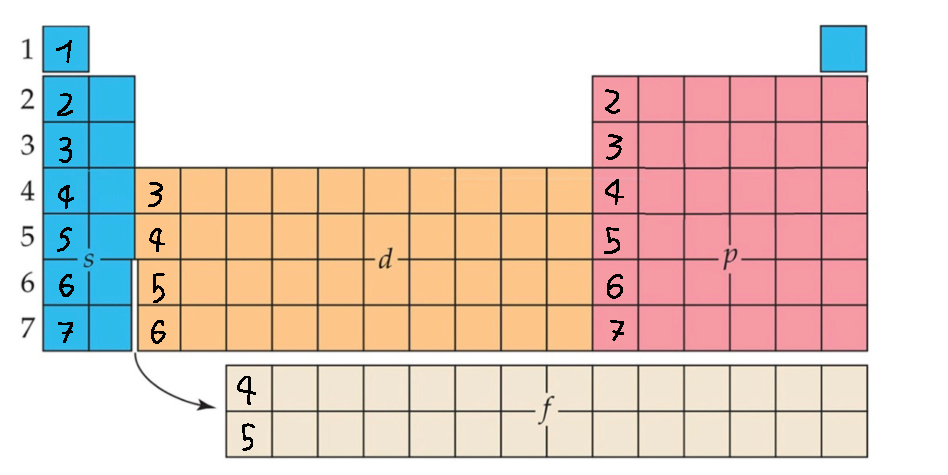
\includegraphics[width=43mm]{src/2_Atoms/images/pse_electron_config.pdf}}
      \end{minipage}
    \end{minipage}
    
    Pauli Exclusion: Each electron has unique set of quantum numbers\\
    Hund's rule: \textbf{Every} orbital in sublevel is first singly occupied\\
    Energy of Hydrogen $e^-$: $E_n = -\frac{hcR_H}{n^2}$, $R_h = 1.097 \cdot 10^7 m^{-1}$\\
    Excitement from shell $n_1$ to $n_2$: $E_H = hcR_H (\frac{1}{n_1^2} - \frac{1}{n_2^2})$

\section{3. Chemical bondings} %Christian
	\input{src/3_Chemical_bondings/3_chemical_bondings}

\section{4. Molecular models}
	\input{src/4_Molecular_models/4_molecular_models}

\section{5. State of matter} %Noa
	\subsection{5.1 Intermolecular forces}
    \begin{enumerate}
        \item \textbf{Hydrogen bonding} (strong)\\
            Entstehen zwischen H und O,N,F Atomen
        \item \textbf{Dipol-Dipol} (mittel) \\
            Sum of all dipole moments from polar bonds in molecule. (molecular dipole) ($\Delta EN>0.5$)
        \item \textbf{Van-der-Waals interactions} (weak)\\
            Entstehen durch temporäre Fluktuationen der Elektronen $\rightarrow$ temporärer Dipol,
            \textbf{Gibts es immer}.Grosse und lange Moleküle haben die stärksten Dispersionskräfte.
    \end{enumerate}

\subsection{5.2 Flüssigkeiten}
    \textbf{Gefrierpunktserniedrigung: } $\Delta T_f=K_fm$\\
    $K_f=$ Kryoskopische Konst.     $m=$ Molalität $\left[\frac{mol}{kg}\right]$\\
    Je tiefer die \textbf{Viskosität}, desto grösser die Mobilität der Moleküle. Viskosität proportional
    zur Stärke der WW. Je höher die Viskosität, desto dickflüssiger. 

\subsection{5.3 Ideale Gase}
    \begin{itemize}
        \item Wir machen 2 Annahmen:
        \begin{itemize}
            \item Gasteilchen wechselwirken nicht.
            \item Gasteilchen haben kein Volumen.
        \end{itemize}
        \item Ideales Gasgesetz: $pV = nRT=N kT$
        \item Dichte $\rho = M\frac{n}{V}=M\frac{p}{RT}$
        \item R ist die universelle Gaskonstante.\vspace*{1mm}
        \item Quadr. Mittelwert der Geschwindigkeit der Gasmoleküle:\\ $u_{rms}=\sqrt{3RT/M}$
        \item $M\left[ gmol^{-1} \right]$, $d\left[ gL^{-1} \right], V\left[L\right]$
    \end{itemize}
    \vspace{1mm}
    Bei hohen Drücken verhalten sich Gase nicht mehr ideal $\rightarrow$  korrigierte
    ideale Gasgleichung:\\\quad\quad$(p+\frac{n^2A}{V^2})(V-nb)=nRT$\\
    \textbf{Partialdruck:} Der Partialdruck ist der Anteil eines Gases am Druck des betrachteten Gasgemisches. Partialdrücke einer Gasmischung sind immer kleiner als der Gesamtdruck.\vspace{0.5mm}\\
    $p_i=n_i\cdot\frac{RT}{V}$ Gesamtdruck $=\Sigma$ aller Partialdrücke



\subsection{5.4 Osmotischer Druck}
    Der Druck der benötigt würde, um Fluss von Lösungsmittelteilchen zu unterdrücken heisst
    osmotischer Druck.
    \begin{equation*}
        \Pi = \left(\frac{n}{V}\right)RT=MRT \text{\quad} M = \text{Molarität}
    \end{equation*}

\section{6. Thermodynamics}
	\input{src/6_Thermodynamics/6_thermodynamics}

\section{7. Kinetics}
	\input{src/7_Kinetics/7_kinetics}

\section{8. Acids and Bases}
	\input{src/8_Acids_and_Bases/8_acids_and_bases}

\section{9. Redox reactions}
	\input{src/9_Redox_rxns/9_redox_rxns}

\end{document}